\documentclass[10pt]{article}
\usepackage[utf8]{inputenc}
\usepackage{pgfplots}
\pgfplotsset{compat=1.15}
\usepackage{mathrsfs}
\usetikzlibrary{arrows}
\pagestyle{empty}

%<<<<<<<WARNING>>>>>>>
% PGF/Tikz doesn't support the following mathematical functions:
% cosh, acosh, sinh, asinh, tanh, atanh,
% x^r with r not integer

% Plotting will be done using GNUPLOT
% GNUPLOT must be installed and you must allow Latex to call external
% programs by adding the following option to your compiler
% shell-escape    OR    enable-write18
% Example: pdflatex --shell-escape file.tex

\begin{document}
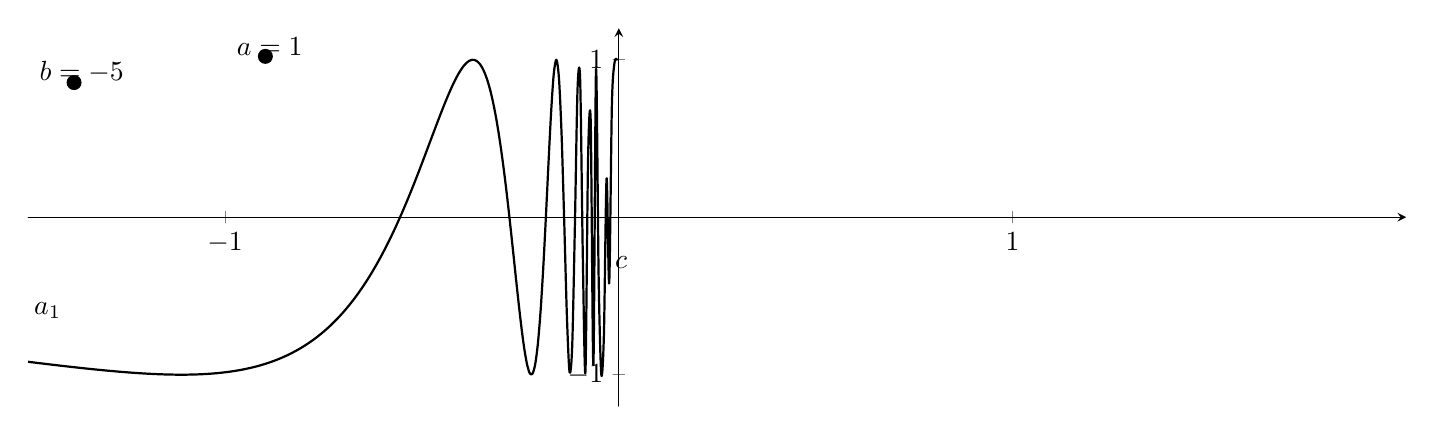
\begin{tikzpicture}[line cap=round,line join=round,>=triangle 45,x=1.0cm,y=1.0cm]
\begin{axis}[x=5.0cm,y=2.0cm,axis lines=middle,xmin=-1.5,xmax=2,
ymin=-1.2,ymax=1.2,xtick={-1,0,1},ytick={-1,0,1}]
%\clip(-1.4872768852614724,-1.2414701334917548) rectangle (2.0720676035159302,1.1223276635030448);
%\draw[line width=4.pt] (-1.2252392541858355,1.0213339931926433) -- (-0.6793275227782584,1.0213339931926433);
\draw[line width=0.8pt, smooth,samples=9000,domain=-6.141592653589793:-0.0001] plot (10*\x,{sin(10/\x)});
%\draw[line width=4.pt] (-1.383553656294033,0.854830915113333) -- (-0.8376419248864558,0.854830915113333);
%\draw[line width=2.pt, smooth,samples=100,domain=0.001:3.141592653589793] plot[parametric] function{t,sin((1/t))};
\begin{scriptsize}
\draw [fill=black] (-0.8976922153412892,1.0213339931926433) circle (2.5pt);
\draw[color=black] (-0.8867739807131376,1.0854786216330332) node {$a = 1$};
\draw[color=black] (-1.450427843391461,-0.5918351731167408) node {$a_{1}$};
\draw [fill=black] (-1.383553656294033,0.854830915113333) circle (2.5pt);
\draw[color=black] (-1.3644467456947678,0.918975543553723) node {$b = -5$};
\draw[color=black] (0.0057917001382510385,-0.29021894151405564) node {$c$};
\end{scriptsize}
\end{axis}
\end{tikzpicture}
\end{document} 